\section{Introduction}

Grâce au HO2, vous avez été réussi à transformer un signal sonore en un signal carré en utilisant principalement un compareteur, un diviseur résistif et un NE555. L'allure de ces signaux est présentée à la Figure~\ref{fig:signal-all}. En principe, votre circuit fonctionne donc comme attendu, bien joué !

\begin{figure}[h!]
    \centering
    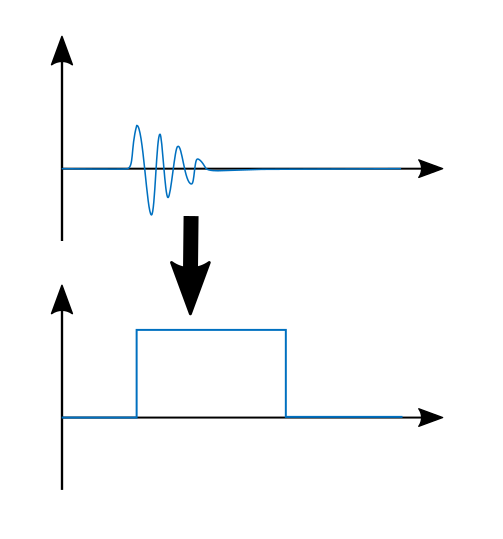
\includegraphics[width=0.5\textwidth]{signals.PNG}
    \caption{Transformation du signal HO2}
    \label{fig:signal-all}
\end{figure}

Maintenant, il va falloir utiliser ce signal carré pour générer le signal de commande: celui-ci doit passer de 0[V] à 5[V] ou de 5[V] à 0[V] lorsqu'un signal carré est généré par un évènement sonore. Vous devez donc reproduire le signal de la Figure~\ref{fig:signal-all_HO3}. Cela vous permettra \textit{in fine} d'utiliser un interrupteur (transitor) connecté à une LED afin de l'allumer ou l'éteindre. Le signal orange à la Figure~\ref{fig:signal-all_HO3} est donc bel et bien votre \textbf{signal de commande}. \\

\begin{figure}[h!]
    \centering
    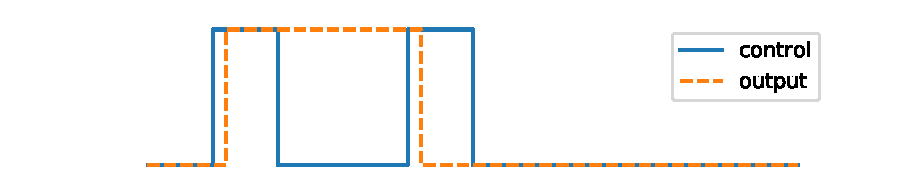
\includegraphics[width=1\textwidth]{figures/signals_control.pdf}
    \caption{Transformation du signal HO3}
    \label{fig:signal-all_HO3}
\end{figure}